% Options for packages loaded elsewhere
\PassOptionsToPackage{unicode}{hyperref}
\PassOptionsToPackage{hyphens}{url}
%
\documentclass[
]{article}
\usepackage{amsmath,amssymb}
\usepackage{iftex}
\ifPDFTeX
  \usepackage[T1]{fontenc}
  \usepackage[utf8]{inputenc}
  \usepackage{textcomp} % provide euro and other symbols
\else % if luatex or xetex
  \usepackage{unicode-math} % this also loads fontspec
  \defaultfontfeatures{Scale=MatchLowercase}
  \defaultfontfeatures[\rmfamily]{Ligatures=TeX,Scale=1}
\fi
\usepackage{lmodern}
\ifPDFTeX\else
  % xetex/luatex font selection
\fi
% Use upquote if available, for straight quotes in verbatim environments
\IfFileExists{upquote.sty}{\usepackage{upquote}}{}
\IfFileExists{microtype.sty}{% use microtype if available
  \usepackage[]{microtype}
  \UseMicrotypeSet[protrusion]{basicmath} % disable protrusion for tt fonts
}{}
\makeatletter
\@ifundefined{KOMAClassName}{% if non-KOMA class
  \IfFileExists{parskip.sty}{%
    \usepackage{parskip}
  }{% else
    \setlength{\parindent}{0pt}
    \setlength{\parskip}{6pt plus 2pt minus 1pt}}
}{% if KOMA class
  \KOMAoptions{parskip=half}}
\makeatother
\usepackage{xcolor}
\usepackage[margin=1in]{geometry}
\usepackage{color}
\usepackage{fancyvrb}
\newcommand{\VerbBar}{|}
\newcommand{\VERB}{\Verb[commandchars=\\\{\}]}
\DefineVerbatimEnvironment{Highlighting}{Verbatim}{commandchars=\\\{\}}
% Add ',fontsize=\small' for more characters per line
\usepackage{framed}
\definecolor{shadecolor}{RGB}{248,248,248}
\newenvironment{Shaded}{\begin{snugshade}}{\end{snugshade}}
\newcommand{\AlertTok}[1]{\textcolor[rgb]{0.94,0.16,0.16}{#1}}
\newcommand{\AnnotationTok}[1]{\textcolor[rgb]{0.56,0.35,0.01}{\textbf{\textit{#1}}}}
\newcommand{\AttributeTok}[1]{\textcolor[rgb]{0.13,0.29,0.53}{#1}}
\newcommand{\BaseNTok}[1]{\textcolor[rgb]{0.00,0.00,0.81}{#1}}
\newcommand{\BuiltInTok}[1]{#1}
\newcommand{\CharTok}[1]{\textcolor[rgb]{0.31,0.60,0.02}{#1}}
\newcommand{\CommentTok}[1]{\textcolor[rgb]{0.56,0.35,0.01}{\textit{#1}}}
\newcommand{\CommentVarTok}[1]{\textcolor[rgb]{0.56,0.35,0.01}{\textbf{\textit{#1}}}}
\newcommand{\ConstantTok}[1]{\textcolor[rgb]{0.56,0.35,0.01}{#1}}
\newcommand{\ControlFlowTok}[1]{\textcolor[rgb]{0.13,0.29,0.53}{\textbf{#1}}}
\newcommand{\DataTypeTok}[1]{\textcolor[rgb]{0.13,0.29,0.53}{#1}}
\newcommand{\DecValTok}[1]{\textcolor[rgb]{0.00,0.00,0.81}{#1}}
\newcommand{\DocumentationTok}[1]{\textcolor[rgb]{0.56,0.35,0.01}{\textbf{\textit{#1}}}}
\newcommand{\ErrorTok}[1]{\textcolor[rgb]{0.64,0.00,0.00}{\textbf{#1}}}
\newcommand{\ExtensionTok}[1]{#1}
\newcommand{\FloatTok}[1]{\textcolor[rgb]{0.00,0.00,0.81}{#1}}
\newcommand{\FunctionTok}[1]{\textcolor[rgb]{0.13,0.29,0.53}{\textbf{#1}}}
\newcommand{\ImportTok}[1]{#1}
\newcommand{\InformationTok}[1]{\textcolor[rgb]{0.56,0.35,0.01}{\textbf{\textit{#1}}}}
\newcommand{\KeywordTok}[1]{\textcolor[rgb]{0.13,0.29,0.53}{\textbf{#1}}}
\newcommand{\NormalTok}[1]{#1}
\newcommand{\OperatorTok}[1]{\textcolor[rgb]{0.81,0.36,0.00}{\textbf{#1}}}
\newcommand{\OtherTok}[1]{\textcolor[rgb]{0.56,0.35,0.01}{#1}}
\newcommand{\PreprocessorTok}[1]{\textcolor[rgb]{0.56,0.35,0.01}{\textit{#1}}}
\newcommand{\RegionMarkerTok}[1]{#1}
\newcommand{\SpecialCharTok}[1]{\textcolor[rgb]{0.81,0.36,0.00}{\textbf{#1}}}
\newcommand{\SpecialStringTok}[1]{\textcolor[rgb]{0.31,0.60,0.02}{#1}}
\newcommand{\StringTok}[1]{\textcolor[rgb]{0.31,0.60,0.02}{#1}}
\newcommand{\VariableTok}[1]{\textcolor[rgb]{0.00,0.00,0.00}{#1}}
\newcommand{\VerbatimStringTok}[1]{\textcolor[rgb]{0.31,0.60,0.02}{#1}}
\newcommand{\WarningTok}[1]{\textcolor[rgb]{0.56,0.35,0.01}{\textbf{\textit{#1}}}}
\usepackage{graphicx}
\makeatletter
\def\maxwidth{\ifdim\Gin@nat@width>\linewidth\linewidth\else\Gin@nat@width\fi}
\def\maxheight{\ifdim\Gin@nat@height>\textheight\textheight\else\Gin@nat@height\fi}
\makeatother
% Scale images if necessary, so that they will not overflow the page
% margins by default, and it is still possible to overwrite the defaults
% using explicit options in \includegraphics[width, height, ...]{}
\setkeys{Gin}{width=\maxwidth,height=\maxheight,keepaspectratio}
% Set default figure placement to htbp
\makeatletter
\def\fps@figure{htbp}
\makeatother
\setlength{\emergencystretch}{3em} % prevent overfull lines
\providecommand{\tightlist}{%
  \setlength{\itemsep}{0pt}\setlength{\parskip}{0pt}}
\setcounter{secnumdepth}{-\maxdimen} % remove section numbering
\ifLuaTeX
  \usepackage{selnolig}  % disable illegal ligatures
\fi
\usepackage{bookmark}
\IfFileExists{xurl.sty}{\usepackage{xurl}}{} % add URL line breaks if available
\urlstyle{same}
\hypersetup{
  pdftitle={Algorithme de Viterbi --- Rapport M2},
  pdfauthor={Mohamed Skander Gharbi},
  hidelinks,
  pdfcreator={LaTeX via pandoc}}

\title{Algorithme de Viterbi --- Rapport M2}
\author{Mohamed Skander Gharbi}
\date{2025-04-10}

\begin{document}
\maketitle

\begin{Shaded}
\begin{Highlighting}[]
\CommentTok{\# Chargement des packages nécessaires}
\FunctionTok{library}\NormalTok{(gtools)}
\end{Highlighting}
\end{Shaded}

\begin{verbatim}
## Warning: package 'gtools' was built under R version 4.4.3
\end{verbatim}

\begin{Shaded}
\begin{Highlighting}[]
\FunctionTok{library}\NormalTok{(ggplot2)}
\end{Highlighting}
\end{Shaded}

\begin{verbatim}
## Warning: package 'ggplot2' was built under R version 4.4.3
\end{verbatim}

\begin{Shaded}
\begin{Highlighting}[]
\FunctionTok{library}\NormalTok{(reshape2)}

\CommentTok{\# Chargement des fonctions définies dans tes scripts}
\FunctionTok{source}\NormalTok{(}\StringTok{"C:/Users/gharb/Documents/M2algo\_viterbi/M2algorithmique\_Viterbi/src/naive\_R/viterbi\_naive.R"}\NormalTok{)}
\end{Highlighting}
\end{Shaded}

\begin{verbatim}
## [1] "Mon premier script Viterbi (version naive)"
## [1] "Pluie"  "Soleil" "Pluie"
\end{verbatim}

\begin{Shaded}
\begin{Highlighting}[]
\FunctionTok{source}\NormalTok{(}\StringTok{"C:/Users/gharb/Documents/M2algo\_viterbi/M2algorithmique\_Viterbi/src/viterbi\_R/viterbi\_algo.R"}\NormalTok{)}
\end{Highlighting}
\end{Shaded}

\begin{verbatim}
## [1] "Pluie"  "Soleil" "Pluie"
\end{verbatim}

\subsection{Introduction}\label{introduction}

Dans le cadre de ce projet, nous étudions l'algorithme de Viterbi, une
méthode classique de programmation dynamique utilisée pour résoudre des
problèmes de reconnaissance de séquences. Cet algorithme est notamment
utilisé dans les modèles de Markov cachés (HMM - Hidden Markov Models),
où l'objectif est de retrouver la séquence d'états cachés la plus
probable ayant généré une suite d'observations.

Nous comparons cette solution optimisée à une approche naïve
(brute-force) qui teste toutes les séquences d'états possibles. Cette
comparaison permettra de mettre en évidence l'intérêt pratique de
l'algorithme de Viterbi.

\begin{center}\rule{0.5\linewidth}{0.5pt}\end{center}

\subsection{Problème étudié}\label{probluxe8me-uxe9tudiuxe9}

On considère un modèle de Markov caché défini par : - Un ensemble
d'états cachés : \(S = \{s_1, s_2, \dots, s_N\}\) - Une séquence
d'observations : \(O = \{o_1, o_2, \dots, o_T\}\) - Une matrice de
transition \(A\) entre états cachés - Une matrice d'émission \(B\)
reliant les états aux observations - Un vecteur de probabilités
initiales \(\pi\)

L'objectif est de trouver la séquence d'états cachés
\(Q = \{q_1, q_2, \dots, q_T\}\) qui maximise la probabilité \(P(Q|O)\),
c'est-à-dire la séquence d'états la plus probable étant donné les
observations.

\begin{center}\rule{0.5\linewidth}{0.5pt}\end{center}

\subsection{Méthodes}\label{muxe9thodes}

\subsubsection{Méthode naïve
(brute-force)}\label{muxe9thode-nauxefve-brute-force}

La méthode naïve consiste à générer \textbf{toutes les combinaisons
possibles} d'états cachés de taille \(T\), puis à calculer leur
probabilité via le modèle HMM.\\
\textbf{Complexité :} \(O(N^T)\)

\begin{Shaded}
\begin{Highlighting}[]
\CommentTok{\# Exemple : exécution de la méthode naïve}
\NormalTok{sequence\_naive }\OtherTok{\textless{}{-}} \FunctionTok{trouver\_sequence\_naive}\NormalTok{(obs, states, pi, A, B)}
\end{Highlighting}
\end{Shaded}

\subsection{Algorithme de Viterbi}\label{algorithme-de-viterbi}

L'algorithme de Viterbi repose sur la programmation dynamique. Il
mémorise à chaque étape les meilleures probabilités d'atteindre chaque
état, ainsi que le chemin correspondant.

Cela permet de réduire considérablement le coût de calcul :\\
Complexité : \(O(N^2 \cdot T)\)

\begin{Shaded}
\begin{Highlighting}[]
\CommentTok{\# Exemple d\textquotesingle{}appel de l’algorithme de Viterbi}
\NormalTok{sequence\_viterbi }\OtherTok{\textless{}{-}} \FunctionTok{viterbi}\NormalTok{(obs, states, pi, A, B)}
\end{Highlighting}
\end{Shaded}

\subsection{Benchmark expérimental}\label{benchmark-expuxe9rimental}

Nous avons réalisé un benchmark sur des séquences d'observations de
taille croissante, afin de comparer le temps d'exécution des deux
méthodes.

\begin{Shaded}
\begin{Highlighting}[]
\FunctionTok{source}\NormalTok{(}\StringTok{"C:/Users/gharb/Documents/M2algo\_viterbi/M2algorithmique\_Viterbi/simulations/benchmark\_tailles.R"}\NormalTok{)}
\end{Highlighting}
\end{Shaded}

\begin{verbatim}
## [1] "Mon premier script Viterbi (version naive)"
## [1] "Pluie"  "Soleil" "Pluie" 
## [1] "Pluie"  "Soleil" "Pluie" 
##   Taille Naif Viterbi
## 1      2 0.00       0
## 2      3 0.00       0
## 3      4 0.00       0
## 4      5 0.00       0
## 5      6 0.00       0
## 6      7 0.00       0
## 7      8 0.00       0
## 8      9 0.01       0
## 9     10 0.01       0
\end{verbatim}

\begin{verbatim}
## Warning: package 'ggplot2' is in use and will not be installed
\end{verbatim}

\begin{verbatim}
## Warning: Using `size` aesthetic for lines was deprecated in ggplot2 3.4.0.
## i Please use `linewidth` instead.
## This warning is displayed once every 8 hours.
## Call `lifecycle::last_lifecycle_warnings()` to see where this warning was
## generated.
\end{verbatim}

\begin{Shaded}
\begin{Highlighting}[]
\FunctionTok{library}\NormalTok{(ggplot2)}
\FunctionTok{library}\NormalTok{(reshape2)}

\NormalTok{df\_long }\OtherTok{\textless{}{-}} \FunctionTok{melt}\NormalTok{(df, }\AttributeTok{id.vars =} \StringTok{"Taille"}\NormalTok{, }\AttributeTok{variable.name =} \StringTok{"Méthode"}\NormalTok{, }\AttributeTok{value.name =} \StringTok{"Temps"}\NormalTok{)}

\FunctionTok{ggplot}\NormalTok{(df\_long, }\FunctionTok{aes}\NormalTok{(}\AttributeTok{x =}\NormalTok{ Taille, }\AttributeTok{y =}\NormalTok{ Temps, }\AttributeTok{color =}\NormalTok{ Méthode)) }\SpecialCharTok{+}
  \FunctionTok{geom\_line}\NormalTok{(}\AttributeTok{size =} \FloatTok{1.2}\NormalTok{) }\SpecialCharTok{+}
  \FunctionTok{geom\_point}\NormalTok{(}\AttributeTok{size =} \DecValTok{2}\NormalTok{) }\SpecialCharTok{+}
  \FunctionTok{labs}\NormalTok{(}
    \AttributeTok{title =} \StringTok{"Temps d\textquotesingle{}exécution selon la taille de la séquence"}\NormalTok{,}
    \AttributeTok{x =} \StringTok{"Taille de la séquence observée"}\NormalTok{,}
    \AttributeTok{y =} \StringTok{"Temps (secondes)"}\NormalTok{,}
    \AttributeTok{color =} \StringTok{"Méthode"}
\NormalTok{  ) }\SpecialCharTok{+}
  \FunctionTok{theme\_minimal}\NormalTok{(}\AttributeTok{base\_size =} \DecValTok{14}\NormalTok{) }\SpecialCharTok{+}
  \FunctionTok{theme}\NormalTok{(}\AttributeTok{plot.title =} \FunctionTok{element\_text}\NormalTok{(}\AttributeTok{hjust =} \FloatTok{0.5}\NormalTok{), }\AttributeTok{legend.position =} \StringTok{"bottom"}\NormalTok{)}
\end{Highlighting}
\end{Shaded}

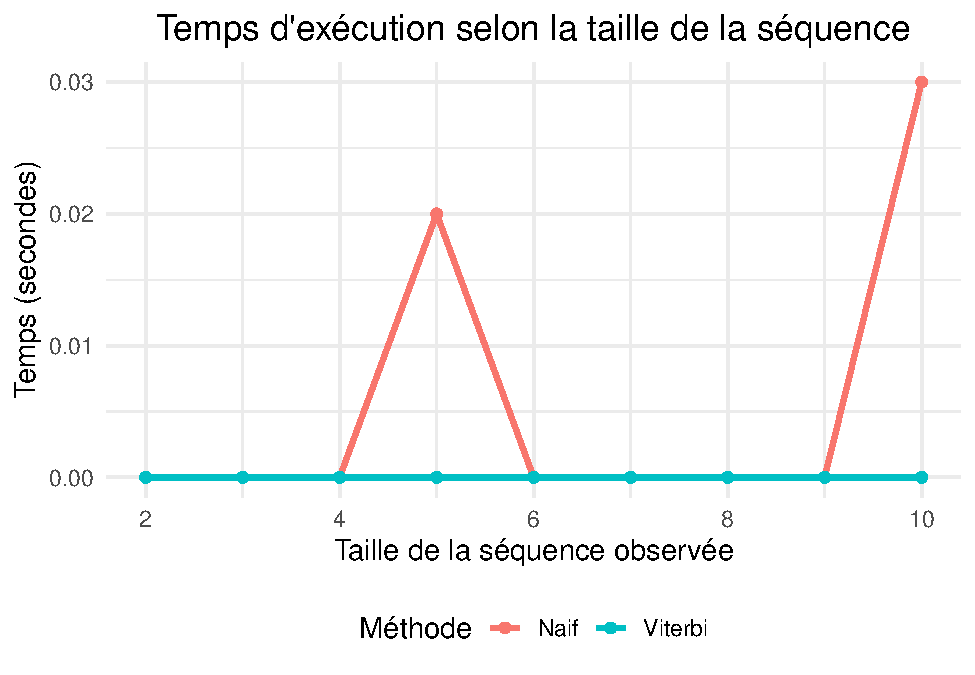
\includegraphics{rapport_viterbi_files/figure-latex/unnamed-chunk-4-1.pdf}
\#\# Analyse des résultats

Le graphique obtenu montre clairement la différence de complexité entre
les deux approches :

La méthode naïve devient rapidement coûteuse lorsque la taille de la
séquence dépasse 7 ou 8 observations.

L'algorithme de Viterbi reste extrêmement rapide, même pour des
séquences plus longues.

Ces résultats confirment les complexités théoriques attendues.

\subsection{Conclusion}\label{conclusion}

Ce projet nous a permis d'implémenter deux approches pour résoudre le
problème de décodage dans un HMM : une version naïve par force brute et
une version optimisée avec l'algorithme de Viterbi.

Les résultats empiriques obtenus montrent l'efficacité du Viterbi en
termes de performance et de scalabilité, en particulier pour des
séquences longues.

Des perspectives d'amélioration incluent :

Une implémentation C++ avec Rcpp

L'application de cet algorithme à des cas réels (reconnaissance vocale,
bioinformatique, traitement automatique du langage, etc.)

\end{document}
